
\section{Force and Motion II\footnote{
1990-93 Dept. of Physics and Astronomy, Dickinson College. Supported by FIPSE
(U.S. Dept. of Ed.) and NSF. Portions of this material have been modified locally
and may not have been classroom tested at Dickinson College.
}}

\makelabheader %(Space for student name, etc., defined in master.tex or labmanual_formatting_commands.tex)

\textbf{Objective} 

To understand the relationship between the direction of the force applied to
an object and the direction of the acceleration of the object. 

\textbf{Overview} 

In the previous lab you examined the one-dimensional motions of an object caused
by a single force applied to the object. You have seen that when friction is
so small that it can be ignored, a single constant applied force will cause
an object to have a constant acceleration. (The object will speed up at a steady
rate.) 

Under these conditions, you have seen that the acceleration is proportional
to the applied force, if the mass of the object is not changed. You saw that
when a constant force is applied to a cart, the cart speeds up at a constant
rate so that it has a constant acceleration. If the applied force is made larger,
then the acceleration is proportionally larger. This allows you to define force
more precisely not just in terms of the stretches of rubber bands and springs,
but as the entity (the ``thing'') that causes acceleration.

The goal of this lab is to continue to develop the relationship between force
and acceleration, an important part of the first two of Newton's famous laws
of motion. You will explore motions in which the applied force (and hence the
acceleration of the object) is in a different direction than the object's velocity.
In this case the object is slowing down in the sense that its speed is decreasing.

\textbf{Apparatus }

\begin{itemize}
\item Pasco 550 Interface
\item Force probe 
\item Variety of hanging masses 
\item Low friction pulley and string 
\item Motion detector 
\item Dynamics cart (with flag) and track 
\item \textit{Capstone} software (\filename{V\_A\_F\_Graphs.cap} experiment file)
\end{itemize}
\textbf{Speeding Up and Slowing Down }

So far you have looked at cases where the velocity, force and acceleration all
have the same sign (all positive). That is, the vectors representing each of
these three vector quantities all point in the same direction. For example,
if the cart is moving toward the right and a force is exerted toward the right,
then the cart will speed up. Thus the acceleration is also toward the right.
The three vectors can be represented as:

\vspace{0.3cm}
{\par\centering 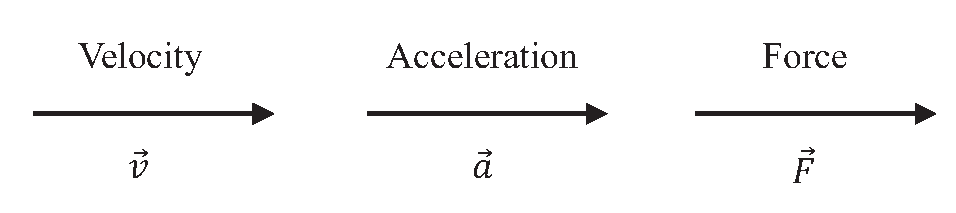
\includegraphics[height=0.7in]{force2/force2_fig1_new.eps} \par}
\vspace{0.3cm}

If the positive x direction is toward the right, then you could also say that
the velocity, acceleration and also force are all positive. In this investigation,
you will examine the vectors representing velocity, force and acceleration for
other motions of the cart. This will be an extension of your earlier observations
of changing motion.

\textbf{Activity 1: Slowing Down} 

Set up the cart, pulley, hanging mass and motion detector as shown below. Now
when you give the cart a push away from the motion detector, it will slow down
after it is released. In this activity you will examine the acceleration and
the applied force.

\vspace{0.3cm}
{\par\centering 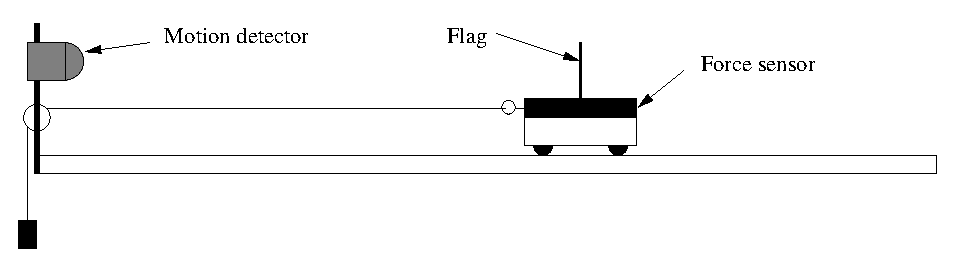
\includegraphics{force2/force2_fig2.eps} \par}
\vspace{0.3cm}

(a) Suppose that you position the cart 0.15 m from the motion detector and give
it a push away from the motion detector and release it. Draw below vectors which
might represent the velocity, force and acceleration of the cart at each time
after it is released and is moving toward the right. Be sure to mark your arrows
with \( {\vec v} \), \( {\vec a} \), or \( {\vec F} \)
as appropriate.

\vspace{0.3cm}
{\par\centering 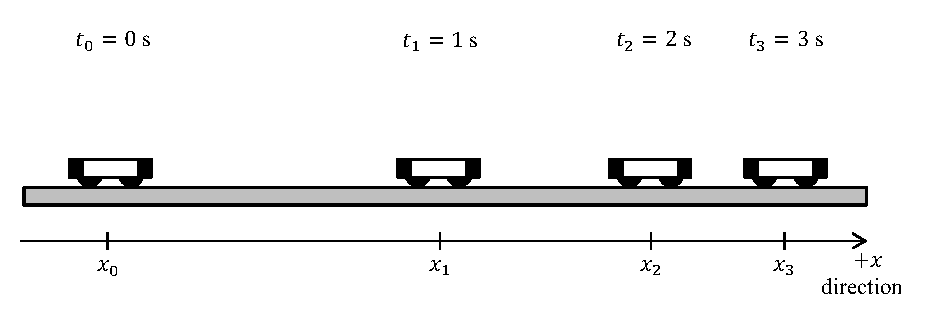
\includegraphics{force2/carts_slowing.eps} \par}
\vspace{0.3cm}

(b) If the positive x direction is toward the right, what are the signs of the
velocity, force and acceleration after the cart is released and is moving toward
the right?
\vspace{10mm}

(c) To test your predictions: 

\begin{enumerate}
\item Open the file \filename{V\_A\_F\_Graphs.cap} in the \filename{\coursefolder} folder.

%\item Calibrate the force probe (see \textit{Calibrating Force Sensors} in \textbf{Appendix \ref{capstone}: Capstone}).
%\textbf{NOTE:} 
%The force sensor and motion detector are looking in opposite directions in 
%this experiment, so when calibrating the force sensor, set the 2nd calibration point to $-1.96$ 
%newtons, so that the force and acceleration will have the same sign.
\item The force sensor and motion detector are looking in opposite directions in this experiment
so we will flip the sign of the force to make the interpretation of your data easier.
To do this  first click on {\tt Hardware Setup} on the left
side of the {\tt Capstone} window, then click the gear symbol on {\tt Forces Sensor Ch A},
and check the box labeled {\tt Change sign}.
To get back out click {\tt OK} and then {\tt Hardware Setup}.


\item Hang a 50-g mass from the end of the string.
\item Test to be sure that the motion detector sees the cart during its complete motion,
and that the string and force probe cable are not interfering with the motion
detector. You may need to move the motion detector to the side slightly so that
it does not see the string. Also make sure that the cables to the motion detector
do not impede the motion of the cart. Remember that the back of the cart must
always be at least 0.15 meter from the motion detector. 
\item Start recording data. When the motion detector starts clicking, give the cart
a short push away from the motion detector and then let it go. Stop the cart
before it reverses its direction. Repeat until you get a good run. 
\item Sketch your velocity, acceleration and force graphs on the axes below. 
%Label the time scale on these axes. 
Indicate with an arrow the time when the push
stopped.
\end{enumerate}
%\vspace{0.3cm}
%{\par\centering 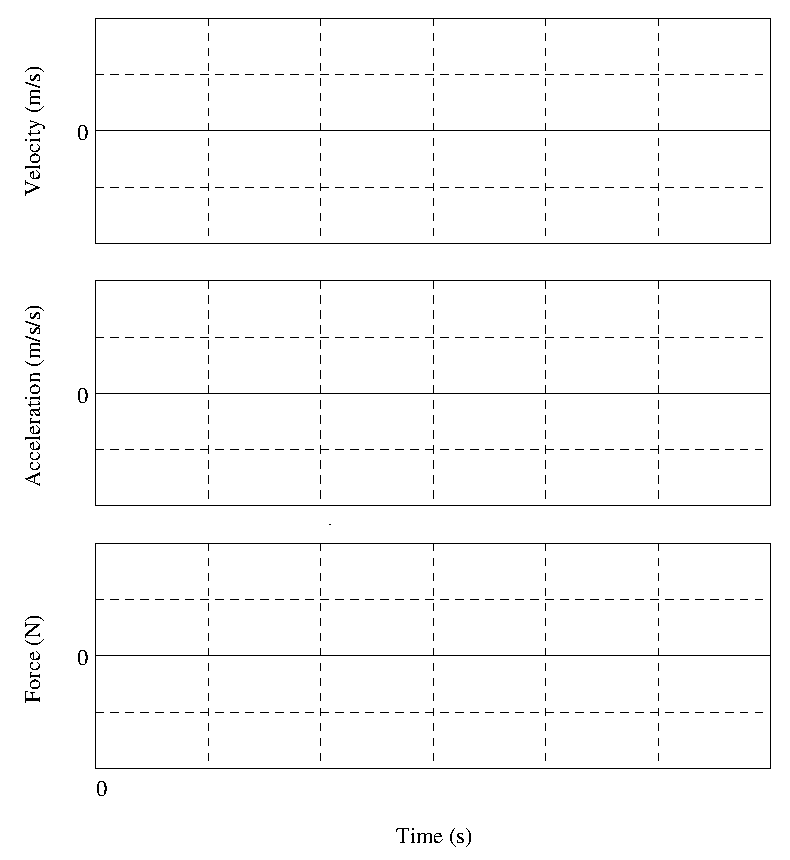
\includegraphics{force2/force2_fig4.eps} \par}
%\vspace{0.3cm}

\begin{lab_groupplot}*{}[lab_grid,
	group style={
		group size=1 by 3,
		xlabels at=edge bottom,
		vertical sep=0.3in,
		},
	width=4.2in,  height=1.4in,
	xlabel=Time (s),
	xmin=0, xmax=12,
	xtick distance = 2, 
	ytick distance = 1, 
	minor tick num=1,
	ytick = {-1,0,1},
	yticklabels = {$-$, 0, $+$},
	]
\nextgroupplot[
	ymin=-1,ymax=1, 
	ylabel={Velocity (m/s)},
	]
\nextgroupplot[
	ymin=-1,ymax=1, 
	ylabel={Acceleration (m/s$^2$)},
	]
\nextgroupplot[
	ymin=-1,ymax=1, 
	ylabel={Force (N)},
	]
\end{lab_groupplot}

(d) Did the signs of the velocity, force and acceleration agree with your predictions?
If not, can you now explain the signs?
\answerspace{30mm}

\pagebreak[3]
(e) Did the velocity and acceleration both have the same sign? Explain these
signs based on the relationship between acceleration and velocity.
\answerspace{20mm}

(f) Did the force and acceleration have the same sign? Were the force and acceleration
in the same direction? Explain.
\answerspace{20mm}

(g) Based on your observations, draw below vectors which might represent the
velocity, force and acceleration for the cart at the same instant in time. Do
these agree with your predictions? If not, can you now explain the directions
of the vectors?
\answerspace{20mm}

(h) After you released the cart, was the force applied by the falling mass constant,
increasing or decreasing?  Why is this kind of force necessary to cause
the observed motion of the cart?
\answerspace{20mm}

\textbf{Activity 2: Speeding Up Toward the Motion Detector }

Using the same setup as in the last activity, you can start with the cart at
the opposite end of the table from the motion detector and release it from rest.
It will then be accelerated toward the motion detector as a result of the force
applied by the falling mass.

(a) Suppose that you release the cart from rest and let it move toward the motion
detector. Draw on the diagram below vectors which might represent the velocity,
force and acceleration of the cart at each time after it is released and is
moving toward the left. Be sure to mark your arrows with $\vec{v}$, $\vec{a}$,
or $\vec{F}$ as appropriate.

\vspace{0.3cm}
{\par\centering 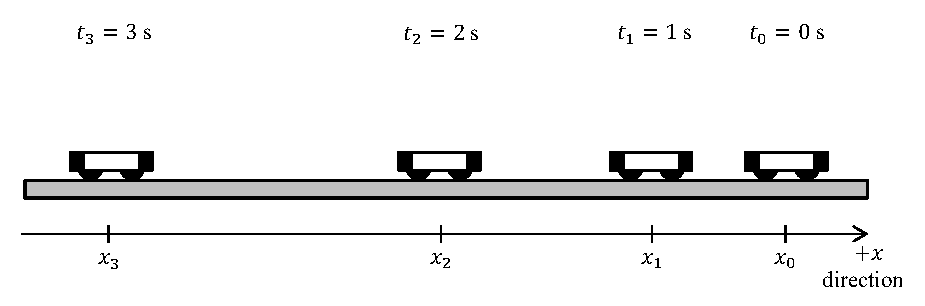
\includegraphics{force2/carts_speeding.eps} \par}
%\vspace{0.3cm}

\pagebreak[3]
(b) What are the signs of the velocity, force and acceleration after the cart
is released and is moving toward the motion detector? (The positive $x$ direction
is toward the right.)
\answerspace{20mm}

(c) Test your predictions. Use a hanging mass of 100 g. Start recording data.
When you hear the motion detector, release the cart from rest as far away from
the motion detector as possible. Catch the cart before it hits the motion detector.
Repeat until you get a good run. Sketch your graphs on the above axes with dashed
lines.

%\pagebreak[2]
(d) Which of the signs -- velocity, force and/or acceleration -- are the same as
in the previous activity (where the cart was slowing down and moving away), and
which are different? Explain any differences in terms of the differences in
the motion of the cart.
\answerspace{20mm}

(e) Based on your observations, draw below vectors which might represent the
velocity, force and acceleration for the cart at the same instant in time. Do
these agree with your predictions? If not, can you now explain the directions
of the vectors?
\answerspace{30mm}

(f) Write down a simple rule in words which describes the relationship between
the direction of the applied force and the direction of the acceleration for
any motion of the cart.
\answerspace{20mm}

(g) Is the direction of the velocity always the same as the direction of the
force? Is the direction of the acceleration always the same as the direction
of the force?
\answerspace{20mm}

\pagebreak[2]
\textbf{Homework }

Questions 1-6 refer to a toy car which can move in either direction along a
horizontal line (the + position axis).

\vspace{0.3cm}
{\par\centering 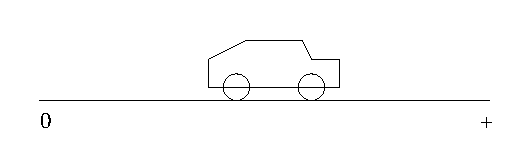
\includegraphics{force2/force2_fig6.eps} \par}
\vspace{0.3cm}

Assume that friction is so small that it can be ignored. Sketch the shape of
the graph of the applied force which would keep the car moving as described
in each statement.

1. The toy car moves away from the origin with a constant velocity.

%\vspace{0.3cm}
%{\par\centering 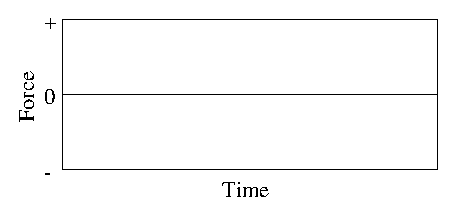
\includegraphics{force2/force2_fig7.eps} \par}
%\vspace{0.3cm}
\begin{lab_axis}*[lab_noticks_2quads,
	width=2.0in,  height=1.2in,
	plus_minus_zero_labels,
	xlabel=Time,
	ylabel=Force,
	]
\end{lab_axis}

2. The toy car moves toward the origin with a constant velocity.

%\vspace{0.3cm}
%{\par\centering 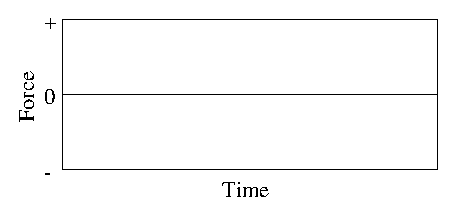
\includegraphics{force2/force2_fig7.eps} \par}
%\vspace{0.3cm}
\begin{lab_axis}*[lab_noticks_2quads,
	width=2.0in,  height=1.2in,
	plus_minus_zero_labels,
	xlabel=Time,
	ylabel=Force,
	]
\end{lab_axis}

3. The toy car moves away from the origin with a steadily decreasing velocity
(a constant acceleration).

%\vspace{0.3cm}
%{\par\centering 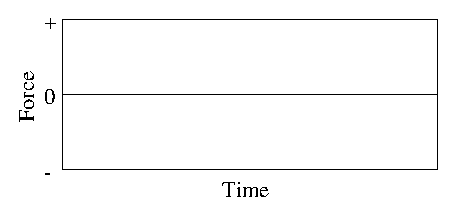
\includegraphics{force2/force2_fig7.eps} \par}
%\vspace{0.3cm}
\begin{lab_axis}*[lab_noticks_2quads,
	width=2.0in,  height=1.2in,
	plus_minus_zero_labels,
	xlabel=Time,
	ylabel=Force,
	]
\end{lab_axis}


4. The toy car moves away from the origin, speeds up and then slows down.

%\vspace{0.3cm}
%{\par\centering 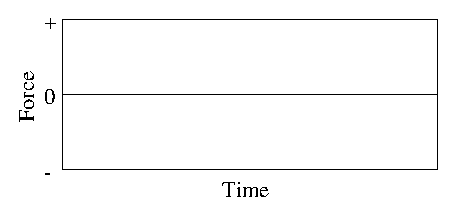
\includegraphics{force2/force2_fig7.eps} \par}
%\vspace{0.3cm}
\begin{lab_axis}*[lab_noticks_2quads,
	width=2.0in,  height=1.2in,
	plus_minus_zero_labels,
	xlabel=Time,
	ylabel=Force,
	]
\end{lab_axis}

5. The toy car moves toward the origin with a steadily increasing speed ( a
constant acceleration).

%\vspace{0.3cm}
%{\par\centering 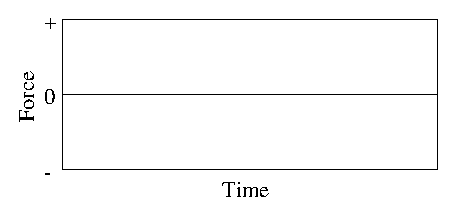
\includegraphics{force2/force2_fig7.eps} \par}
%\vspace{0.3cm}
\begin{lab_axis}*[lab_noticks_2quads,
	width=2.0in,  height=1.2in,
	plus_minus_zero_labels,
	xlabel=Time,
	ylabel=Force,
	]
\end{lab_axis}

6. The toy car is given a push away form the origin and released. It continues
to move with a constant velocity. sketch the force after the car is released.

%\vspace{0.3cm}
%{\par\centering 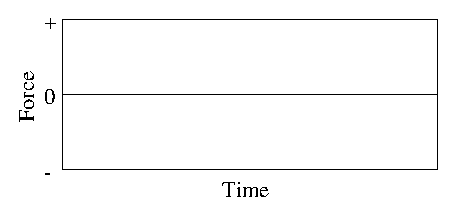
\includegraphics{force2/force2_fig7.eps} \par}
%\vspace{0.3cm}
\begin{lab_axis}*[lab_noticks_2quads,
	width=2.0in,  height=1.2in,
	plus_minus_zero_labels,
	xlabel=Time,
	ylabel=Force,
	]
\end{lab_axis}

7. A cart is moving toward the right and speeding up, as shown in the diagram
below. Draw arrows above the cart representing the magnitudes and directions
of the net (combined) forces you think are needed on the cart at the times shown
to maintain its motion with a steadily increasing velocity.

\vspace{0.3cm}
{\par\centering 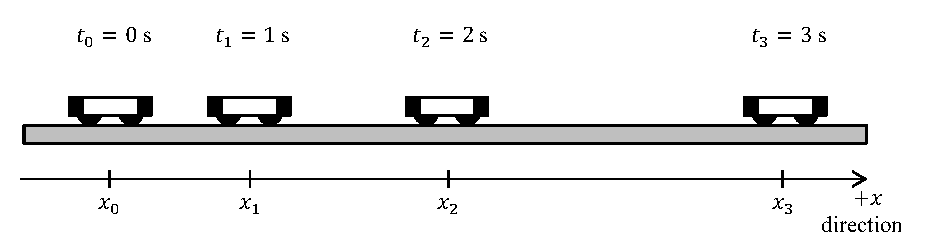
\includegraphics{force2/carts_speeding_hw1.eps} \par}
\vspace{0.3cm}

Explain the reasons for your answers.
\answerspace{20mm}

8. If the positive direction is toward the right, what is the sign of the force
at $t = 2$ sec in question 7? Explain.
\answerspace{20mm}

\pagebreak[2]
9. A cart is moving toward the right and slowing down, as shown in the diagrams
below. Draw arrows above the cart representing the magnitudes and directions
of the net (combined) forces you think are needed on the cart at $t = 0$ s, 
$t
= 1$ s, etc. to maintain its motion with a steadily decreasing velocity.

\vspace{0.3cm}
{\par\centering 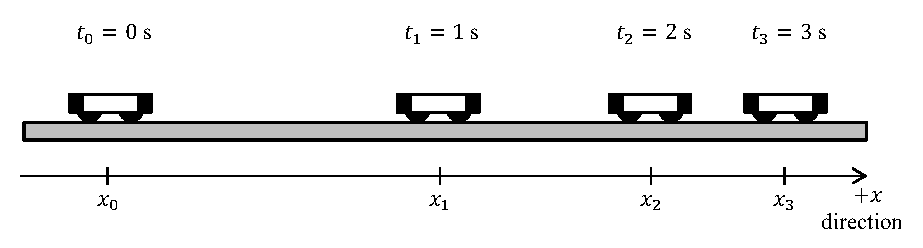
\includegraphics{force2/carts_slowing_hw2.eps} \par}
\vspace{0.3cm}

Explain the reasons for your answers.
\answerspace{25mm}

10. If the positive direction is toward the right, what is the sign of the force
at $t = 2$ sec in question 9? Explain.
\answerspace{25mm}

\pagebreak[2]
11. A toy car can move in either direction along a horizontal line (the + position
axis).

\vspace{0.3cm}
{\par\centering 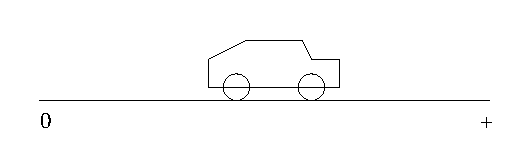
\includegraphics{force2/force2_fig6.eps} \par}
\vspace{0.3cm}

Assume that friction is so small that it can be ignored. A force toward the
right of constant magnitude is applied to the car. Sketch on the axes below
using a solid line the shape of the acceleration-time graph of the car.

%\vspace{0.3cm}
%{\par\centering 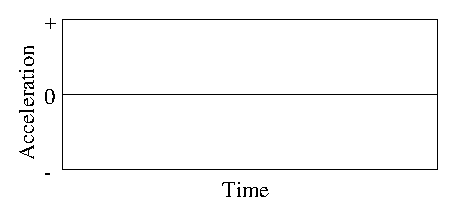
\includegraphics{force2/force2_fig10.eps} \par}
%\vspace{0.3cm}
\begin{lab_axis}*[lab_noticks_2quads,
	width=2.0in,  height=1.2in,
	plus_minus_zero_labels,
	xlabel=Time,
	ylabel=Acceleration,
	]
\end{lab_axis}

Explain the shape of your graph in terms of the applied force.

